\documentclass[12pt, a4paper]{extarticle}
\usepackage{GOST}
\usepackage{array}
\usepackage{verbatim}
\usepackage[detect-all]{siunitx}
\usepackage{amsmath}
\usepackage{amssymb}
\usepackage[utf8]{inputenc}
\usepackage{hyperref}
\usepackage{float}
\makeatletter
\renewcommand\@biblabel[1]{#1.}
\makeatother

\usepackage{listings}
\lstset{ 
	language=C,
	basicstyle=\small\sffamily, 
	numbers=left, 
	numberstyle=\tiny,
	stepnumber=1,
	numbersep=5pt,
	showspaces=false,            
	showstringspaces=false,      
	showtabs=false,             
	frame=single,            % рисовать рамку вокруг кода
	tabsize=4,      
	commentstyle=\color{green},
	keywordstyle=\color{blue}\textbf,
	numberstyle=\scriptsize\color{gray}, % the style that is used for the line-numbers
	rulecolor=\color{black},
	captionpos=t,
	breaklines=true,         % автоматически переносить строки 
	breakatwhitespace=false, % переносить строки по пробелу
	escapeinside={\#*}{*)} 
}
\graphicspath{{images/}}

\begin{document}
\begin{table}[ht]
	\centering
	\begin{tabular}{|c|p{400pt}|} 
	\hline
		\begin{tabular}[c]{@{}c@{}} 
\includegraphics[scale=0.8]{b_logo} \\\end{tabular} &
		\footnotesize\begin{tabular}[c]{@{}c@{}}\textbf{Министерство~науки~и~высшего~образования~Российской~Федерации}\\\textbf{Федеральное~государственное~бюджетное~образовательное~учреждение}\\\textbf{~высшего~образования}\\\textbf{«Московский~государственный~технический~университет}\\\textbf{имени~Н.Э.~Баумана}\\\textbf{(национальный~исследовательский~университет)»}\\\textbf{(МГТУ~им.~Н.Э.~Баумана)}\\\end{tabular}  \\
	\hline
	\end{tabular}
\end{table}
\noindent\rule{\textwidth}{4pt}
\noindent\rule[14pt]{\textwidth}{1pt}
\hfill 
\noindent
\makebox{ФАКУЛЬТЕТ~}%
\makebox[\textwidth][l]{\underline{~~~~~«Информатика и системы управления»~~~~~~~~~~~~~~~~~~~~~~~~~}}%
\\
\noindent
\makebox{КАФЕДРА~}%
\makebox[\textwidth][l]{\underline{«Программное обеспечение ЭВМ и информационные технологии»}}%

\begin{center}
	\vspace{1.5cm}
	{\bf\huge Расчетно-пояснительная записка\par}
	{\bf\Large к курсовой работе\par}
	\vspace{0cm}
\end{center}


\noindent
\makebox{\large{\bf Тема:}~~~}
\makebox[\textwidth][l]{\large\underline{~Разработка протокола с дедупликацией~~~~~~~~~~~~~}}\\

\noindent
\makebox{\large{\bf Дисциплина:}~~~}
\makebox[\textwidth][l]{\large\underline{~Компьютерные сети~~~~~~~~~~~~~~~~~~~~}}\\

\vspace{1cm}
\noindent
\begin{tabular}{l c c c c c}
    Студент      & ~ИУ7-75Б~       & \hspace{2.5cm} & \hspace{3cm}               & &  П.К Хетагуров \\\cline{2-2}\cline{4-4} \cline{6-6} 
    \hspace{3cm} & {\footnotesize(Группа)} &                & {\footnotesize(Подпись, дата)} & & {\footnotesize(И.О. Фамилия)}
\end{tabular}

\vspace{0.5cm}

\noindent
\begin{tabular}{l c c c c}
    Руководитель проекта & \hspace{3.3cm}   & \hspace{3.5cm}              & & Н.О. Рогозин \\\cline{3-3} \cline{5-5} 
    \hspace{2.9cm}  &              & {\footnotesize(Подпись, дата)} & & {\footnotesize(И.О. Фамилия)}
\end{tabular}

\begin{center}	
	\vfill
	\large \textit {Москва, 2021}
\end{center}

\thispagestyle {empty}
\pagebreak

\section*{Задание}
\begin{enumerate}
\item Присвоить портам устройств статические ipv4 адреса в соответствии с вариантом
\item Настроить безопасный доступ к коммутаторам и маршрутизатору
\item Указать адреса портов маршрутизатора как адрес шлюза по умолчанию для конечных узлов
\item Настроить DNS сервер
\item Указать адрес DNS сервера для конечных узлов
\item Настроить почтовый сервер SMTP и POP3
\item Добавить почтовые записи на DNS - сервер 
\item Настроить почтовый клиент на всех ПК
\item Настроить HTTP сервер, разместить там тестовую страницу с номером варианта, фамилией, номером группы, датой выполнения работы.
\item Проверить корректное прохождение сигнала между всеми узлами сети, доступность   
настроенных сервисов со стороны клиентов на ПК 
\item Отметить широковещательные домены и домены коллизий на схеме
 \end{enumerate}
Адрес ПК (сеть 1): 10.1.x.y 255.255.255.0 
Адрес DNS сервера (сеть 2): 192.168.x.y 255.255.255.0
Адрес HTTP и SMTP серверов (сеть 3): 172.16.x.y 255.255.255.0

x - Ваш номер по списку в Электронном Университете, y -порядковый номер от 1 и выше


\newpage
\section{Результаты}
\begin{figure}[H]
	\centering
	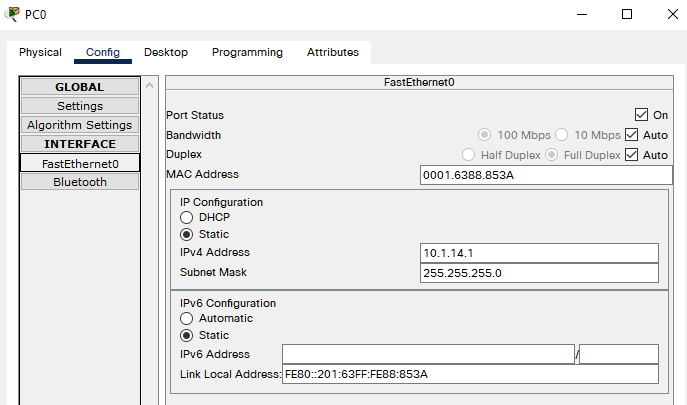
\includegraphics[scale=0.7]{images/pc1.png}
	\caption{Настройка интерфеса}
\end{figure}

\begin{figure}[H]
	\centering
	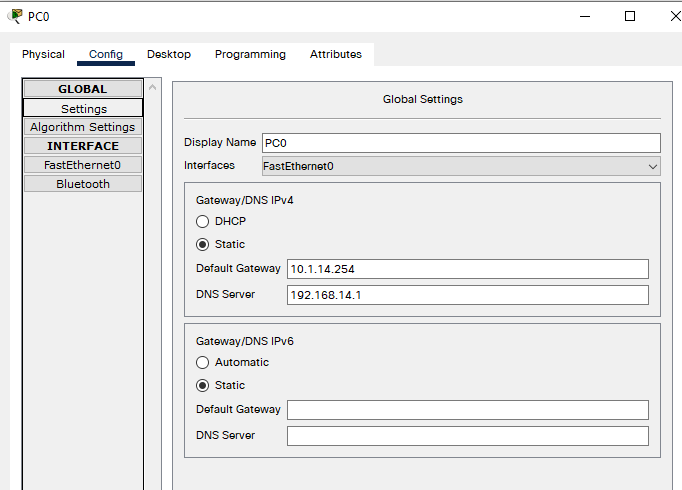
\includegraphics[scale=0.7]{images/pc2.png}
	\caption{Настройка дефолтного шлюза}
\end{figure}

\begin{figure}[H]
	\centering
	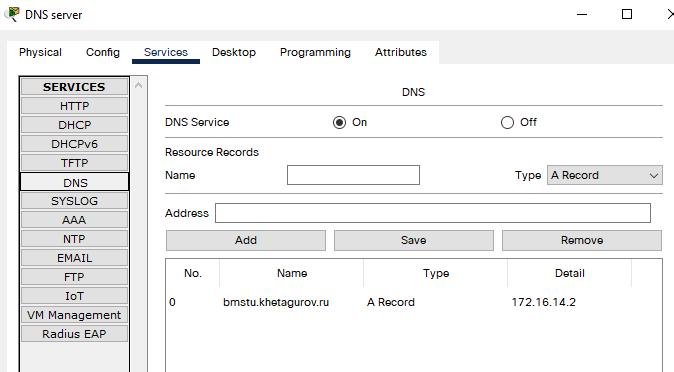
\includegraphics[scale=0.7]{images/dns.png}
	\caption{Настройка DNS}
\end{figure}

\begin{figure}[H]
	\centering
	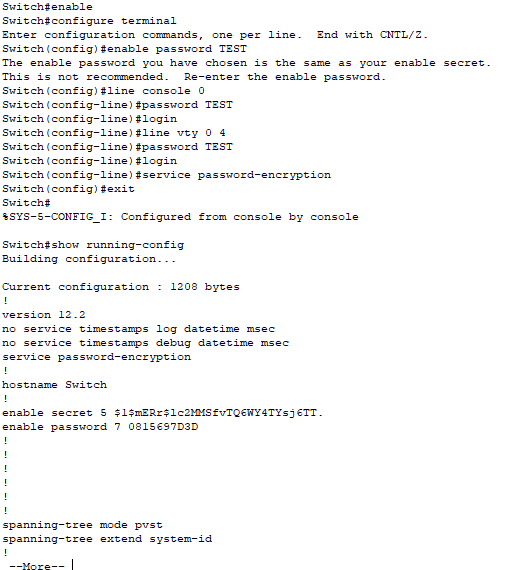
\includegraphics[scale=0.7]{images/sec.png}
	\caption{Настройка безопасного доступа}
\end{figure}

\begin{figure}[H]
	\centering
	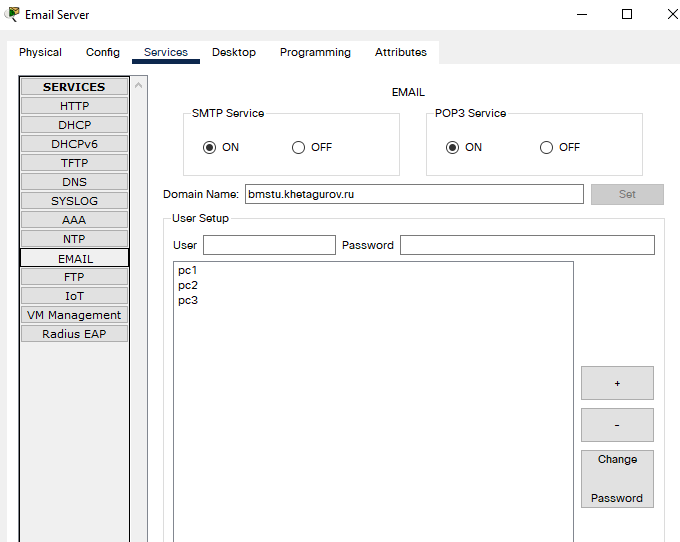
\includegraphics[scale=0.7]{images/smtp.png}
	\caption{Настройка SMTP-сервера}
\end{figure}

\begin{figure}[H]
	\centering
	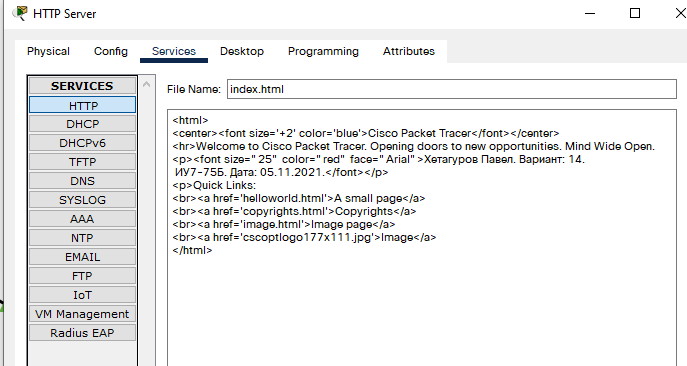
\includegraphics[scale=0.7]{images/http.png}
	\caption{Изменение страницы на HTTP-сервере}
\end{figure}

\begin{figure}[H]
	\centering
	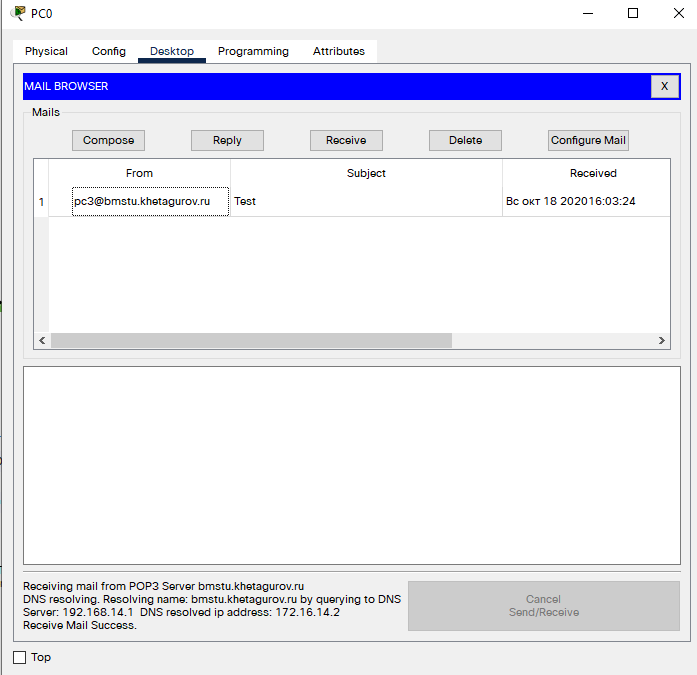
\includegraphics[scale=0.7]{images/smtp-check.png}
	\caption{Проверка SMTP-сервера}
\end{figure}

\begin{figure}[H]
	\centering
	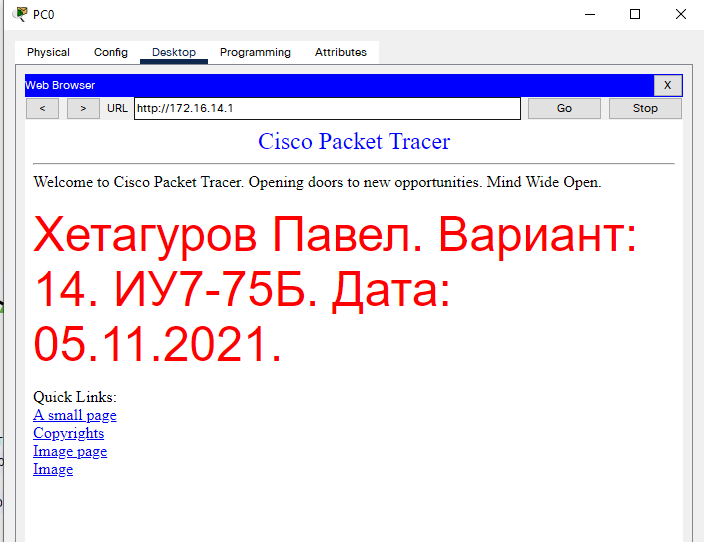
\includegraphics[scale=0.7]{images/http-check.png}
	\caption{Проверка HTTP-сервера}
\end{figure}

Домены. Красным - широковещательные, синим - домены коллизий.
\begin{figure}[H]
	\centering
	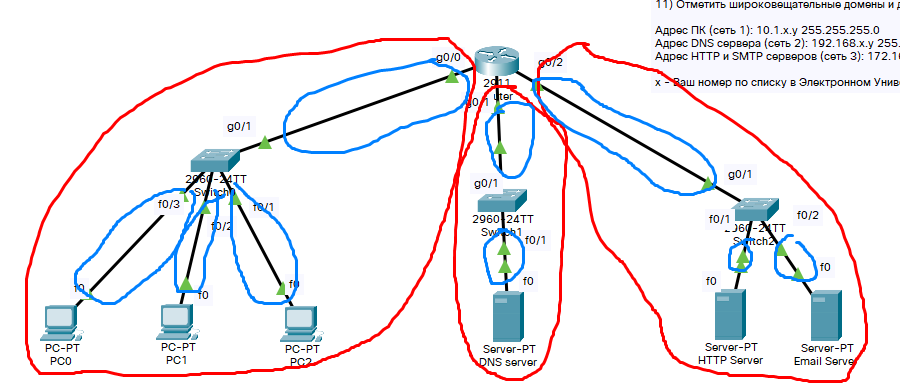
\includegraphics[scale=0.7]{images/domens.png}
	\caption{Домены}
\end{figure}

\end{document}




